
\pagebreak
\section{Phụ lục}
\appendix

\section{Các bước triển khai}

\subsection{Cài đặt Greenplum}

Đầu tiên cần thiết lập SSH cho các máy chủ segment trong Greenplum.
Tạo khóa SSH trên máy chủ Coordinator:

\begin{mdframed}[backgroundcolor=white, linecolor=black, roundcorner=5pt]
\begin{alltt}
ssh-keygen -t rsa -b 4096 -C "gpadmin@master"
\end{alltt}
\end{mdframed}

Sao chép khóa SSH tới các máy chủ segment:


\begin{mdframed}[backgroundcolor=white, linecolor=black, roundcorner=5pt]
\begin{alltt}
sudo nano ~/.ssh/authorized_keys
\end{alltt}
\end{mdframed}

Trước khi cài đặt Greenplum, cần phải cài đặt các gói phụ trợ cần thiết để đảm bảo môi trường hoạt động tốt. Lệnh sau để cài đặt các gói này với đúng phiên bản yêu cầu:

\begin{mdframed}[backgroundcolor=white, linecolor=black, roundcorner=5pt]
\begin{alltt}
sudo apt install -y 
libzstd-dev=1.4.4+dfsg-3ubuntu0.1
pkg-config=0.29.1-0ubuntu4
python3-pip=20.0.2-5ubuntu1.10
libpq-dev=12.19-0ubuntu0.20.04.1
libreadline-dev=8.0-4
bison=2:3.5.1+dfsg-1
libxml2-dev=2.9.10+dfsg-5ubuntu0.20.04.7
zlib1g-dev=1:1.2.11.dfsg-2ubuntu1.5
libcurl4-openssl-dev=7.68.0-1ubuntu2.23
libbz2-dev=1.0.8-2 libyaml-dev=0.2.2-1
libevent-dev=2.1.11-stable-1
libperl-dev=5.30.0-9ubuntu0.8
python3-dev=3.8.2-0ubuntu2
libkrb5-dev=1.17-6ubuntu4.6
libapr1-dev=1.6.5-1ubuntu1
libxerces-c-dev=3.2.2+debian-1ubuntu0.2
\end{alltt}
\end{mdframed}


Sau đó, cài đặt các thư viện Python cần thiết:

\begin{mdframed}[backgroundcolor=white, linecolor=black, roundcorner=5pt]
\begin{alltt}
pip install psycopg2==2.9.9 psutil==6.0.0
\end{alltt}
\end{mdframed}

Tải mã nguồn Greenplum từ GitHub và di chuyển vào thư mục gpdb-archive vừa tải về:

\begin{mdframed}[backgroundcolor=white, linecolor=black, roundcorner=5pt]
\begin{alltt}
git clone https://github.com/Greenplum-db/gpdb-archive.git
cd gpdb-archive
\end{alltt}
\end{mdframed}

Tiến hành biên dịch mã nguồn và cài đặt Greenplum:
\begin{mdframed}[backgroundcolor=white, linecolor=black, roundcorner=5pt]
\begin{alltt}
make -j8 
sudo make -j8 install
\end{alltt}
\end{mdframed}

Chạy lệnh sau để cấu hình Greenplum với các tùy chọn phù hợp:

\begin{mdframed}[backgroundcolor=white, linecolor=black, roundcorner=5pt]
\begin{alltt}
./configure --with-perl --with-python --with-libxml --with-gssapi --prefix=/usr/local/gpdb
\end{alltt}
\end{mdframed}

Thiết lập môi trường cho Greenplum:

\begin{mdframed}[backgroundcolor=white, linecolor=black, roundcorner=5pt]
\begin{alltt}
source /usr/local/gpdb/Greenplum_path.sh
\end{alltt}
\end{mdframed}



Sao chép các tệp cấu hình cần thiết:

\begin{mdframed}[backgroundcolor=white, linecolor=black, roundcorner=5pt]
\begin{alltt}
cp $GPHOME/docs/cli_help/gpconfigs/gpinitsystem_config .
cp $GPHOME/docs/cli_help/gpconfigs/hostfile_gpinitsystem .
\end{alltt}
\end{mdframed}

Trước khi khởi tạo hệ thống Greenplum cần xuất biến môi trường MASTER\_DATA\_DIRECTORY để chỉ định thư mục lưu trữ dữ liệu của master:

\begin{mdframed}[backgroundcolor=white, linecolor=black, roundcorner=5pt]
\begin{alltt}
export MASTER_DATA_DIRECTORY=/home/gpadmin/data/master/gpseg-1
\end{alltt}
\end{mdframed}


Mở tệp gpinitsystem\_config và cấu hình các tham số như sau:

\begin{mdframed}[backgroundcolor=white, linecolor=black, roundcorner=5pt]
\begin{alltt}
SEG_PREFIX=gpseg
PORT_BASE=6000
COORDINATOR_HOSTNAME=master
declare -a DATA_DIRECTORY=(/data1/primary /data1/primary /data1/primary/data2/primary)
COORDINATOR_DIRECTORY=/home/gpadmin/data/master
COORDINATOR_PORT=5432
TRUSTED_SHELL=ssh
ENCODING=UNICODE
MACHINE_LIST_FILE=/hostfile_gpinitsystem
\end{alltt}
\end{mdframed}


Cấu hình này xác định các tham số quan trọng cho hệ thống Greenplum. SEG\_PREFIX=gpseg đặt tiền tố cho các thư mục dữ liệu của các segment, giúp quản lý dễ dàng. PORT\_BASE=6000 chỉ định cổng bắt đầu cho các segment chính, với cổng đầu tiên là 6000. Coordinator được chỉ định bởi COORDINATOR\_HOSTNAME=master, với dữ liệu được lưu tại COORDINATOR\_DIRECTORY=/data/master và kết nối qua cổng COORDINATOR\_PORT=5432. Thư mục dữ liệu của các segment được chỉ định trong DATA\_DIRECTORY, với các đường dẫn lưu trữ cụ thể. TRUSTED\_SHELL=ssh xác định sử dụng SSH để đảm bảo các kết nối từ xa an toàn, và ENCODING=UNICODE đảm bảo hỗ trợ ký tự đa ngôn ngữ trong cơ sở dữ liệu. Cuối cùng, MACHINE\_LIST\_FILE=/hostfile\_gpinitsystem chứa danh sách các máy chủ trong cụm, giúp thiết lập kết nối giữa chúng.

Cấu hình IP của các segment trong tệp hostfile\_gpinitsystem

Chạy lệnh sau để khởi tạo hệ thống Greenplum với các cấu hình đã thiết lập:

\begin{mdframed}[backgroundcolor=white, linecolor=black, roundcorner=5pt]
\begin{alltt}
gpinitsystem -c gpinitsystem_config
\end{alltt}
\end{mdframed}

Các bước trên đã hướng dẫn chi tiết cách chuẩn bị, cài đặt và cấu hình hệ thống Greenplum trên Ubuntu phiên bản 20.04. Quy trình này bao gồm việc cài đặt các gói cần thiết, tải và cài đặt Greenplum, thiết lập SSH cho các segment, cấu hình và khởi tạo hệ thống Greenplum, cũng như thêm đường dẫn của MASTER\_DATA\_DIRECTORY và khởi động hệ thống Greenplum.



\subsection{Tích hợp provider sử dụng cho Greenplum}

Để tích hợp ASP.NET Membership với cơ sở dữ liệu Greenplum cần sử dụng provider của Devart là dotConnect for PostgreSQL. Quá trình này bao gồm việc tạo schema cần thiết trên Greenplum và cấu hình các provider trong file Web.config.

Đầu tiên cần truy cập vào trang chủ của Devart và tải schema mẫu dành cho ASP.NET Membership. Sau khi tải xuống, hãy tạo schema này trên cơ sở dữ liệu Greenplum.

Đầu tiên cần kết nối với Greenplum trong file Web.config.


\begin{mdframed}[backgroundcolor=white, linecolor=black, roundcorner=5pt]
\begin{alltt}
<add name="PgSqlServices" 
     connectionString="Server=IP_server;
                       Port=Port_Server;
                       Database=Name_Database;
                       User Id=IP_server;
                       Password=Password_server;"/>
</connectionStrings>
\end{alltt}
\end{mdframed}

Dưới đây là các cấu hình cần thiết trong file Web.config để sử dụng ASP.NET Membership, Roles, và Profile với Greenplum thông qua provider của Devart.

Cấu hình ASP.NET Membership
\begin{mdframed}[backgroundcolor=white, linecolor=black, roundcorner=5pt]
\begin{alltt}
<membership defaultProvider="AspNetPgSqlMembershipProvider"
            userIsOnlineTimeWindow="15">
  <providers>
    <add
      name="AspNetPgSqlMembershipProvider"
      type="Devart.Data.PostgreSql.Web.Providers.PgSqlMembershipProvider,
            Devart.Data.PostgreSql.Web, Version=8.3.20, Culture=neutral,
            PublicKeyToken=09af7300eec23701"
      connectionStringName="PgSqlServices"
      enablePasswordRetrieval="false"
      enablePasswordReset="true"
      requiresQuestionAndAnswer="true"
      requiresUniqueEmail="false"
      passwordFormat="Hashed"
      maxInvalidPasswordAttempts="5"
      passwordAttemptWindow="10" />
  </providers>
</membership>
\end{alltt}
\end{mdframed}

Cấu hình ASP.NET Role
\begin{mdframed}[backgroundcolor=white, linecolor=black, roundcorner=5pt]
\begin{alltt}
<roleManager defaultProvider="AspNetPgSqlRoleProvider"
             enabled="true"
             cacheRolesInCookie="true"
             cookieName=".ASPROLES"
             cookieTimeout="30"
             cookiePath="/"
             cookieProtection="All">
  <providers>
    <add
      name="AspNetPgSqlRoleProvider"
      type="Devart.Data.PostgreSql.Web.Providers.PgSqlRoleProvider,
            Devart.Data.PostgreSql.Web, Version=8.3.20, Culture=neutral,
            PublicKeyToken=09af7300eec23701"
      connectionStringName="PgSqlServices" />
  </providers>
</roleManager>
\end{alltt}
\end{mdframed}

Cấu hình ASP.NET Profile 
\begin{mdframed}[backgroundcolor=white, linecolor=black, roundcorner=5pt]
\begin{alltt}
<profile defaultProvider="AspNetPgSqlProfileProvider">
  <providers>
    <add
      name="AspNetPgSqlProfileProvider"
      type="Devart.Data.PostgreSql.Web.Providers.PgSqlProfileProvider,
            Devart.Data.PostgreSql.Web, Version=8.3.20, Culture=neutral,
            PublicKeyToken=09af7300eec23701"
      connectionStringName="PgSqlServices" />
  </providers>
  <properties>
    <add name="FirstName" />
    <add name="LastName" />
    <add name="DateOfBirth" type="System.DateTime"/>
  </properties>
</profile>
\end{alltt}
\end{mdframed}

Việc sử dụng dotConnect for PostgreSQL của Devart cho phép dễ dàng tích hợp ASP.NET Membership với cơ sở dữ liệu Greenplum. Quá trình này bao gồm việc tạo schema cần thiết và cấu hình các provider trong file Web.config.


\subsection{Dữ liệu}

\subsubsection{Chuẩn bị dữ liệu}

Dữ liệu này bao gồm thông tin về thành viên, quyền hạn, hồ sơ cá nhân và các giao dịch liên quan. Thông tin thành viên bao gồm: UserID, UserName, Email, Password, IsApproved, IsLockedOut, LastLoginDate, CreationDate. Quyền hạn bao gồm: RoleID, RoleName. Hồ sơ cá nhân bao gồm: FirstName, LastName, DateOfBirth, SecurityQuestion, SecurityAnswer.

Mã nguồn chuẩn bị dữ liệu kiểm thử:

\begin{mdframed}[backgroundcolor=white, linecolor=black, roundcorner=5pt]
\begin{alltt}
SeedUsers()
\{
    var random = new Random();
    int attempt = 5;
    for (int i = 0; i < 500000; i++)
    \{
        bool isLocked = random.Next(2) == 1;
        var userName = $"member{i}";
        var password = $"Password123!";
        var email = $"user{i}@example.com";
        MembershipCreateStatus createStatus;
        MembershipUser newUser = Membership.CreateUser(
            userName, password, email,
            "What is your favorite color?", "Blue",
            isApproved: true, null, out createStatus);

        if (createStatus == MembershipCreateStatus.Success)
        \{
            if (isLocked)
            \{
                SimulateFailedLogins(userName, attempt);
            \}

            AssignUserToRandomRole(userName);

            try
            \{
                SaveUserProfile(userName, $"FirstName{i}", $"LastName{i}");
            \}
            catch (Exception profileEx)
            \{
                Console.WriteLine($"Error saving profile for user {userName}: {profileEx}");
            \}
        \}
        else
        \{
            Console.WriteLine(\$"Error creating user {userName}: {createStatus}");
        \}
    \}
\}

SimulateFailedLogins(string userName, int attempts)
\{
    for (int attempt = 0; attempt < attempts; attempt++)
    \{
        Membership.ValidateUser(userName, "wrongPassword");
    \}
\}

AssignUserToRandomRole(string userName)
\{
    var random = new Random();
    string[] roles = \{ "Admin", "User" \};
    string role = roles[random.Next(roles.Length)];
    Roles.AddUserToRole(userName, role);
\}

SaveUserProfile(string userName, string firstName, string lastName)
\{
    dynamic profile = ProfileBase.Create(userName, true);
    profile.SetPropertyValue("FirstName", firstName);
    profile.SetPropertyValue("LastName", lastName);
    profile.SetPropertyValue("DateOfBirth", new DateTime(1990, 1, 1)
    .AddDays(new Random().Next(365)));
    profile.Save();
\}
\end{alltt}
\end{mdframed}

Trong đó:

SeedUsers: Hàm chính để tạo thành viên. Với mỗi thành viên, nó sẽ tạo thông tin cơ bản như userName, password, và email. Sau đó, gọi hàm Membership.CreateUser để tạo thành viên.
SimulateFailedLogins: Giả lập các lần đăng nhập thất bại để khóa tài khoản thành viên.
AssignUserToRandomRole: Gán thành viên vào một quyền hạn ngẫu nhiên.
SaveUserProfile: Lưu hồ sơ cá nhân của thành viên, bao gồm FirstName, LastName, và DateOfBirth.

\subsubsection{Chuyển dữ liệu}

Trong quá trình chuyển đổi dữ liệu từ MSSQL sang Greenplum, PDI được sử dụng để thực hiện các thao tác ETL (Extract, Transform, Load). Dưới đây là các bước chi tiết cho quá trình này.

Đầu tiên cần kết nối MSSQL và Greenplum trong phần Database connection PDI như hình \ref{fig:ConMSSQL}, \ref{fig:ConGreenplum}.


\begin{figure}
    \centering
    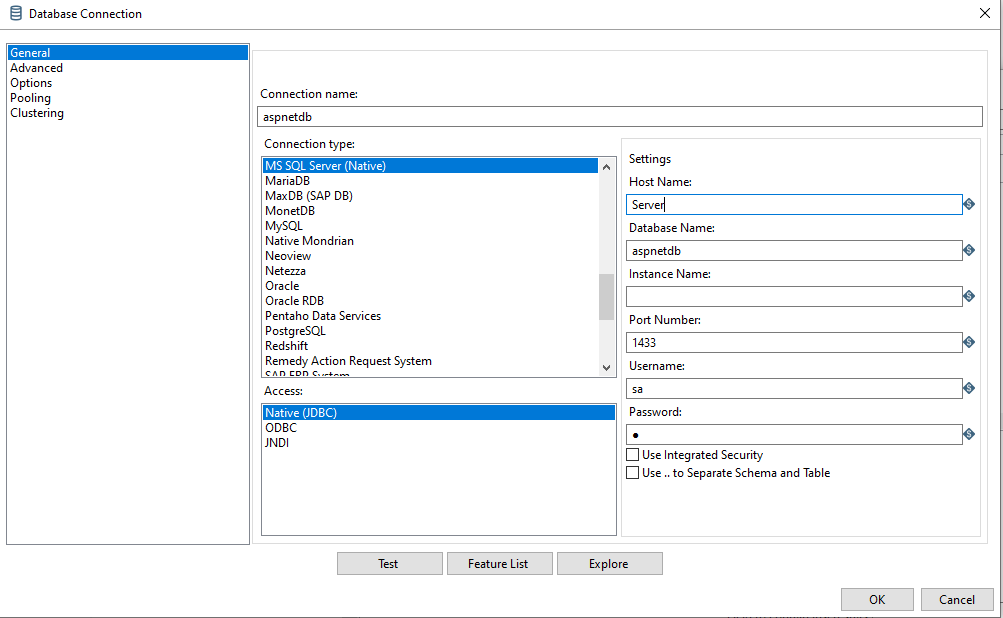
\includegraphics[width=0.8\linewidth]{ConMSSQL.png}
    \caption{Kết nối PDI với MSSQL}
    \label{fig:ConMSSQL}
\end{figure}


\begin{figure}
    \centering
    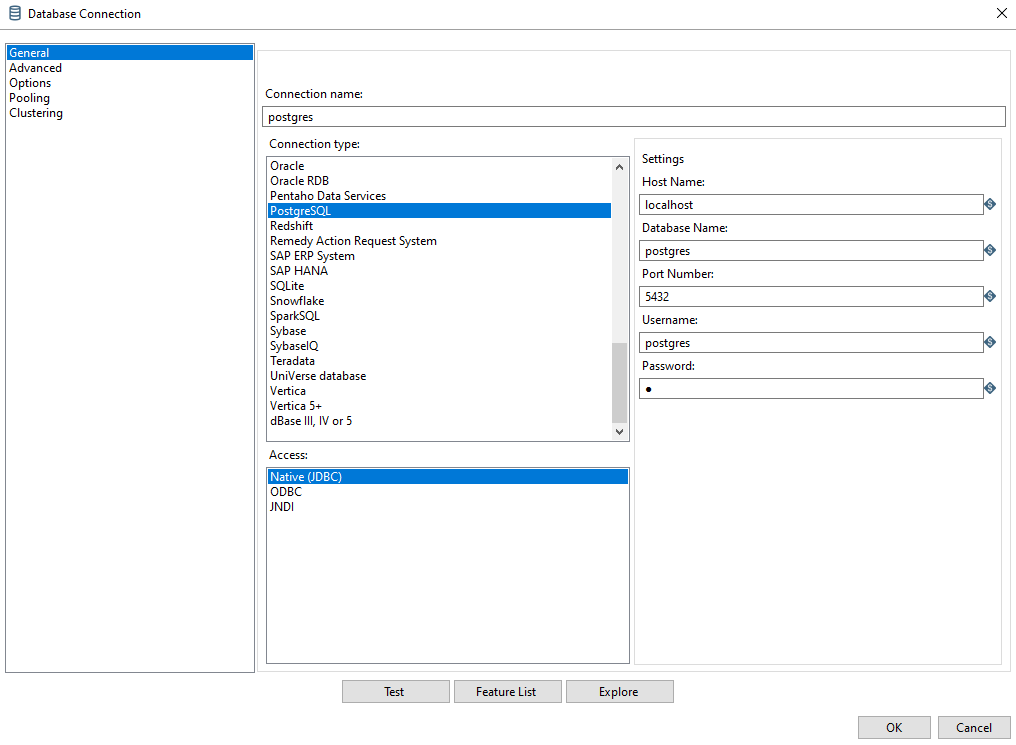
\includegraphics[width=0.8\linewidth]{ConGreenplum.png}
    \caption{Kết nối PDI với Greenplum}
    \label{fig:ConGreenplum}
\end{figure}

\begin{figure}
    \centering
    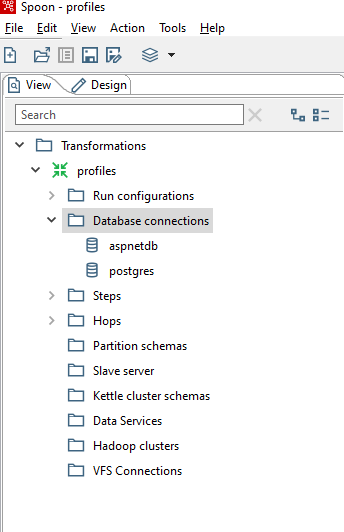
\includegraphics[width=0.8\linewidth]{ComMSGL.png}
    \caption{Kết nói thành công MSSQL và Greenplum}
    \label{fig:ComMSGL}
\end{figure}



Hình \ref{fig:ComMSGL} khi kết nối thành công MSSQL và Greenplum 


Quá trình chuyển dữ liệu bằng Pentaho được thực hiện qua các bước chính sau đây:

Khởi đầu quá trình bằng việc thiết lập một bản thiết kế tổng quát cho quy trình ETL trong Pentaho. Mục tiêu là tạo ra một luồng công việc tự động, bao gồm các bước từ truy vấn dữ liệu từ nguồn MSSQL, xử lý và chuyển đổi dữ liệu, đến việc tải dữ liệu vào đích Greenplum.

Sử dụng công cụ Table Input của Pentaho để truy vấn và trích xuất dữ liệu từ cơ sở dữ liệu MSSQL. Các truy vấn SQL được sử dụng để lấy dữ liệu từ các bảng như roles, users, usersinroles và membership.

Hình \ref{fig:roles} sử dụng Table Input để lấy thông tin role trong bảng aspnet\_Roles

\begin{figure}
    \centering
    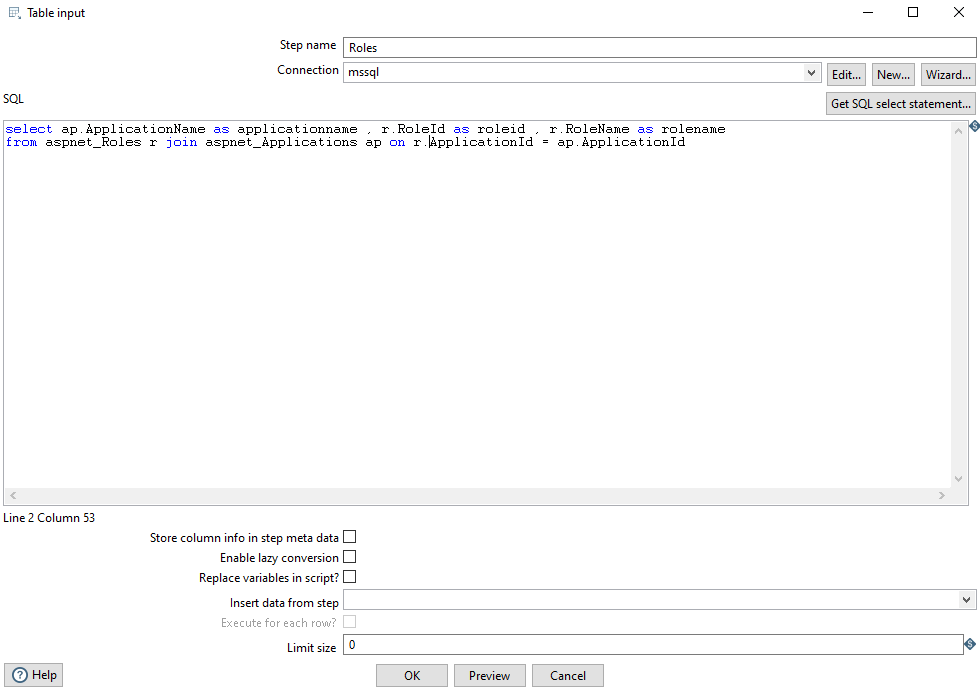
\includegraphics[width=0.8\linewidth]{roles.png}
    \caption{Table Input của aspnet\_Roles của MSSQL}
    \label{fig:roles}
\end{figure}

Hình \ref{fig:usersl} sử dụng Table Input để lấy thông tin users trong bảng aspnet\_Users

\begin{figure}
    \centering
    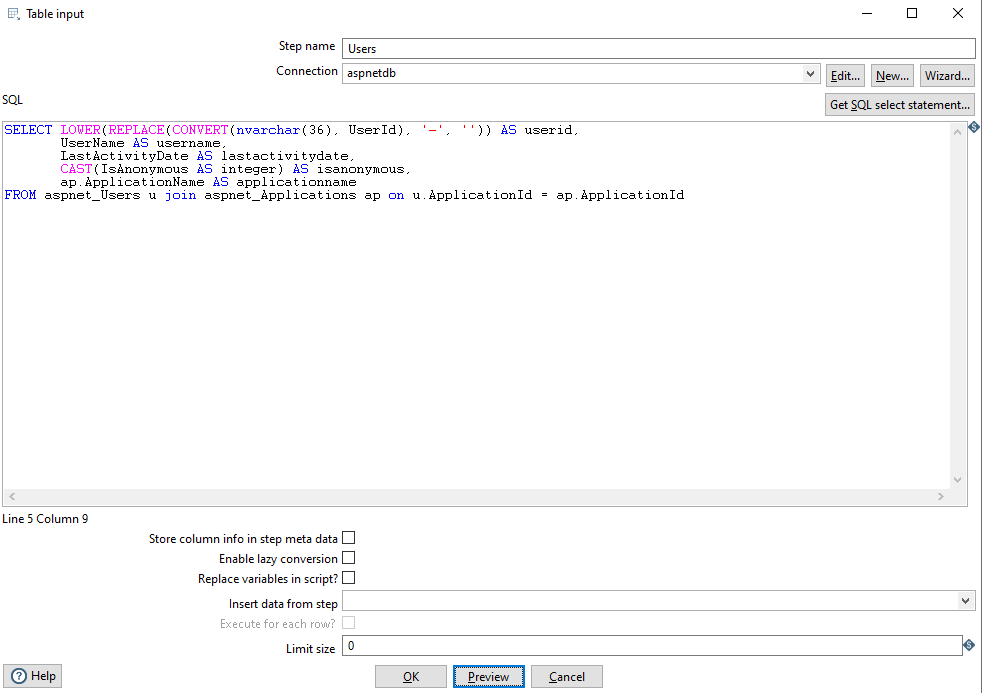
\includegraphics[width=0.8\linewidth]{users.png}
    \caption{Table Input của aspnet\_Users của MSSQL}
    \label{fig:usersl}
\end{figure}

Hình \ref{fig:UsersInRoles} sử dụng Table Input để lấy thông tin role trong bảng aspnet\_UsersInRoles

\begin{figure}
    \centering
    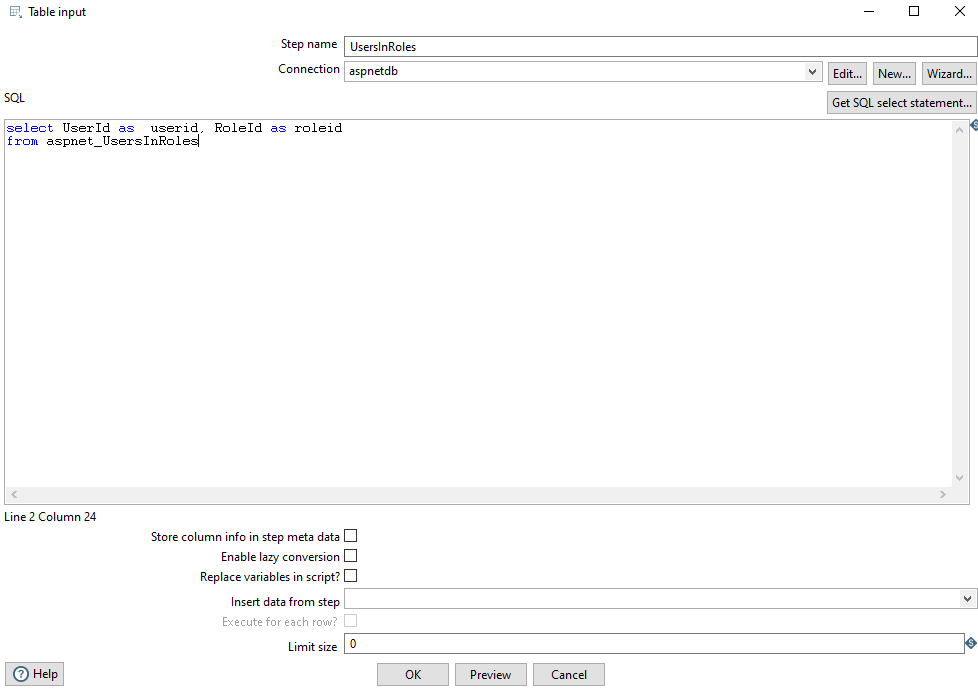
\includegraphics[width=0.8\linewidth]{UsersInRoles.png}
    \caption{Table Input của aspnet\_UsersInRoles của MSSQL}
    \label{fig:UsersInRoles}
\end{figure}

Hình \ref{fig:Membership} sử dụng Table Input để lấy thông tin Membership trong bảng aspnet\_Membership

\begin{figure}
    \centering
    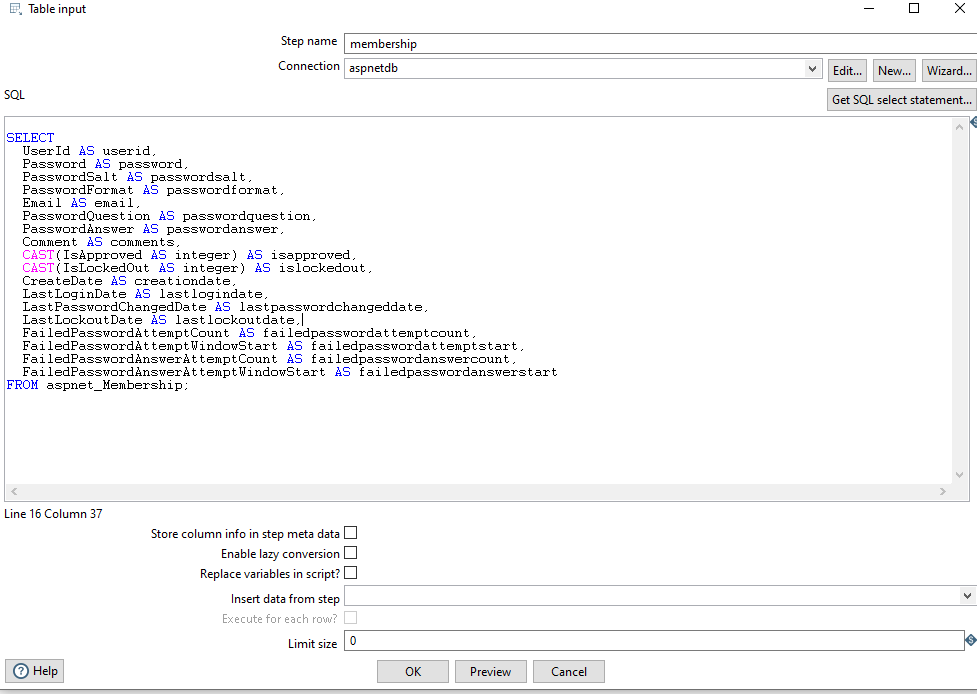
\includegraphics[width=0.8\linewidth]{Membership.png}
    \caption{Table Input của aspnet\_Membership của MSSQL}
    \label{fig:Membership}
\end{figure}


Sử dụng công cụ Execute SQL script của Pentaho để nhận dữ liệu từ các bảng như aspnet\_roles, aspnet\_users, aspnet\_usersinroles, và aspnet\_membership.

Hình \ref{fig:groles} sử dụng Execute SQL script để lấy thông tin roles trong bảng aspnet\_roles của Greenplum


\begin{figure}
    \centering
    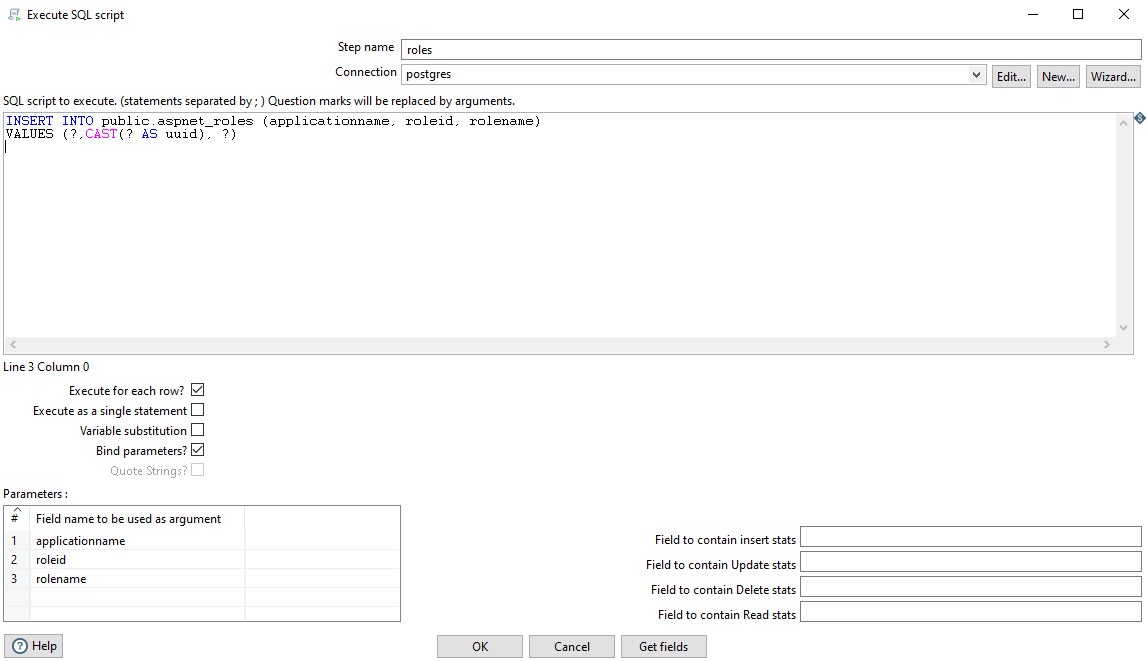
\includegraphics[width=0.8\linewidth]{groles.png}
     \caption{Execute SQL script aspnet\_roles của Greenplum}
    \label{fig:groles}
\end{figure}

Hình \ref{fig:bulk_users1} sử dụng PostgreSQL bulk loader để lấy thông tin users trong bảng aspnet\_users của Greenplum


\begin{figure}
    \centering
    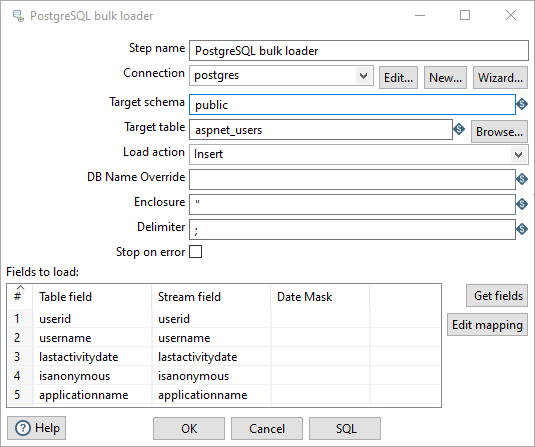
\includegraphics[width=0.8\linewidth]{bulk_users1.png}
     \caption{PostgreSQL bulk loader aspnet\_users của Greenplum}
    \label{fig:bulk_users1}
\end{figure}

Hình \ref{fig:Bulk_uir} sử dụng PostgreSQL bulk loader để lấy thông tin usersinroles trong bảng aspnet\_usersinroles của Greenplum


\begin{figure}
    \centering
    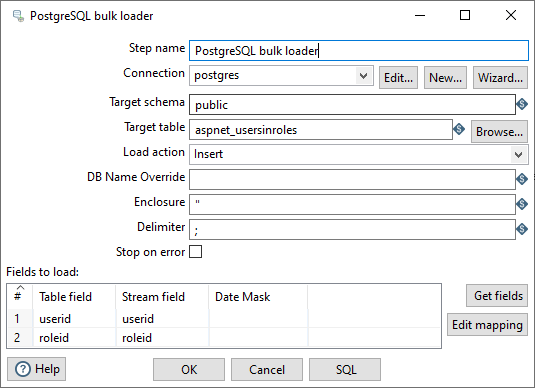
\includegraphics[width=0.8\linewidth]{Bulk_uir.png}
    \caption{PostgreSQL bulk loader aspnet\_usersinroles của Greenplum}
    \label{fig:Bulk_uir}
\end{figure}


Hình \ref{fig:bulk_mem} sử dụng Execute SQL script để lấy thông tin membership trong bảng aspnet\_membership của Greenplum


\begin{figure}
    \centering
    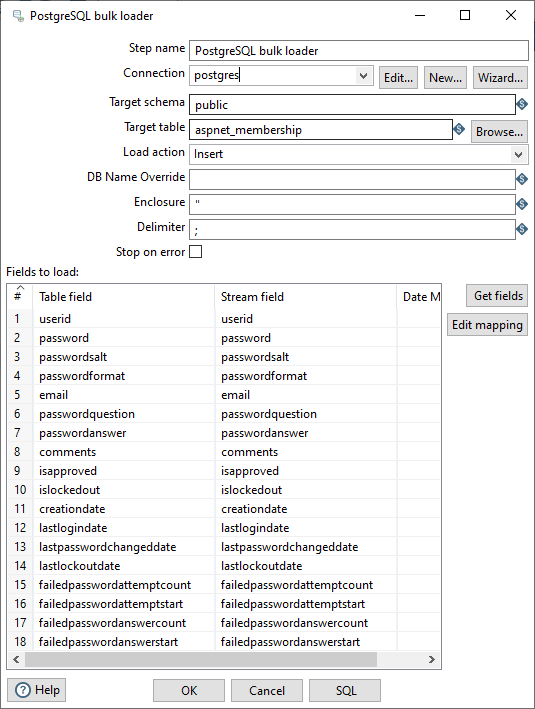
\includegraphics[width=0.8\linewidth]{bulk_mem.png}
     \caption{Execute SQL script aspnet\_membership của Greenplum}
    \label{fig:bulk_mem}
\end{figure}






Cuối cùng như hình \ref{fig:job} sử dụng Job để sử dụng các transformation để hoàn chỉnh ETL của PDI


\begin{figure}
    \centering
    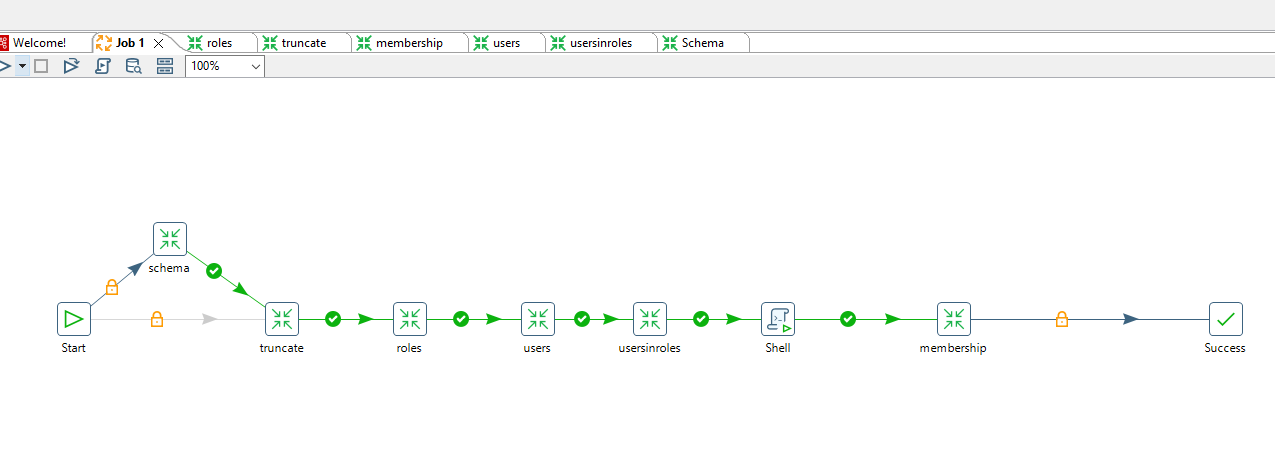
\includegraphics[width=0.8\linewidth]{jobcom.png}
    \caption{Job ETL}
    \label{fig:job}
\end{figure}


\subsection{Giao diện}



Như hình \ref{fig:day} hiển thị thống kê thành viên trong hệ thống ASP.NET Membership cung cấp cái nhìn tổng quan về số lượng thành viên và tình trạng tài khoản. Thẻ "Members" màu xanh hiển thị tổng số lượng thành viên và thẻ "Blocked" màu đỏ hiển thị số lượng thành viên bị khóa, giúp quản trị viên dễ dàng theo dõi và quản lý. Biểu đồ dạng đường hiển thị số lượng thành viên đăng nhập hàng ngày trong tháng 6/2024. Bộ lọc thời gian (Day, Week, Month, Year) giúp linh hoạt trong việc phân tích dữ liệu. Giao diện này hỗ trợ quản lý hiệu quả, phân tích xu hướng và phát hiện, xử lý các vấn đề liên quan đến tài khoản thành viên, đảm bảo hệ thống hoạt động ổn định và hiệu quả.




Hình ảnh \ref{fig:list} thể hiện giao diện quản lý thành viên trong hệ thống ASP.NET Membership. Giao diện lọc thành viên theo các tiêu chí khác nhau như đăng nhập gần đây, bị khóa, và không đăng nhập trong tháng qua. Dữ liệu hiển thị trên bảng bao gồm thông tin số thứ tự, tên đăng nhập, họ, tên, email và lần đăng nhập cuối cùng của thành viên.

\subsection{Kiểm thử}

Để cài đặt Apache JMeter truy cập trang chủ Apache JMeter\footnote{\url{https://jmeter.apache.org/download_jmeter.cgi}} và tải phiên bản mới nhất dưới dạng file ZIP hoặc TGZ. Sau khi giải nén file đã tải về vào một thư mục trên máy tính, cần cài đặt Java Development Kit (JDK) bằng cách tải từ trang chủ Oracle JDK\footnote{\url{https://www.oracle.com/java/technologies/downloads/}}, chạy file cài đặt và thiết lập biến môi trường JAVA\_HOME trỏ tới thư mục cài đặt JDK. ví dụ: \begin{verbatim}C:\Program Files\Java\jdk-11\end{verbatim}

Chạy file jmeter.bat (trên Windows) hoặc jmeter (trên Unix/Linux) để khởi động giao diện người dùng của JMeter.

Trong JMeter, Thread Group là thành phần cốt lõi, nơi xác định số lượng người dùng ảo (threads) sẽ tương tác đồng thời với hệ thống. Để thêm Thread Group, chọn Add > Threads (Users) > Thread Group.

Listeners trong JMeter đóng vai trò quan trọng trong việc theo dõi, ghi nhận và trực quan hóa kết quả kiểm thử. Để thêm Listener vào Thread Group, chọn Add > Listener > Summary Report, Aggregate Report, View Results Tree như hình \ref{fig:testjmeter}.


\begin{figure}
    \centering
    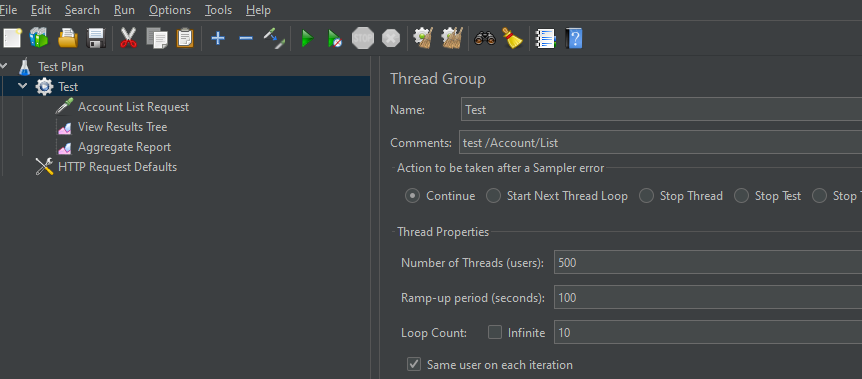
\includegraphics[width=0.8\linewidth]{testjmeter.png}
    \caption{Thông số thread group trong JMeter}
    \label{fig:testjmeter}
\end{figure}

\begin{figure}
    \centering
    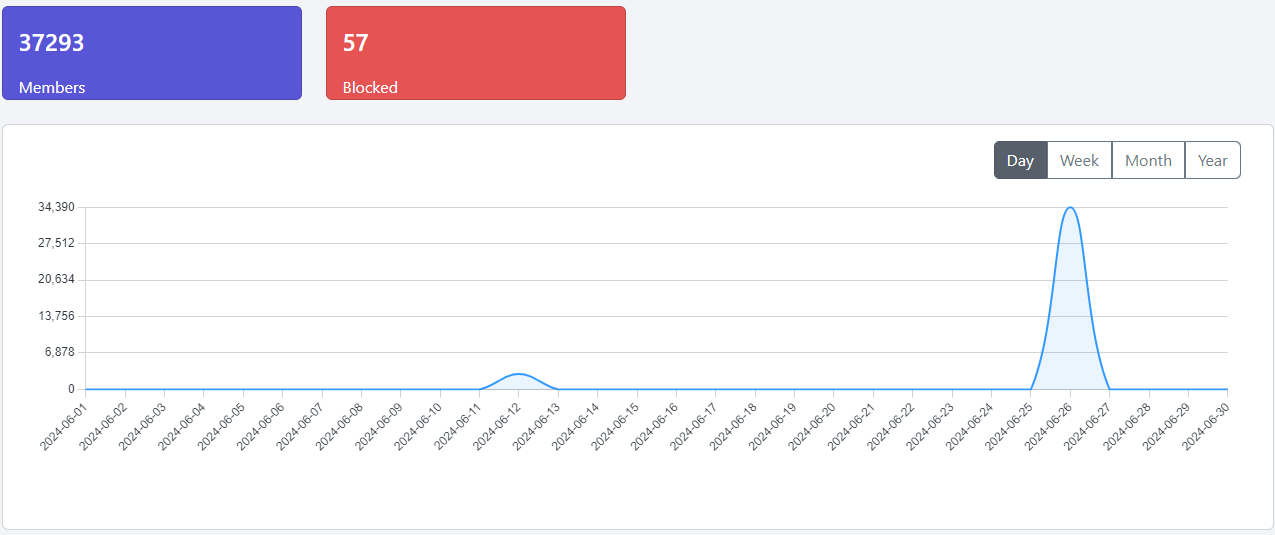
\includegraphics[width=0.8\linewidth]{day.png}
    \caption{Giao diện hiển thị thống kê thành viên trong hệ thống ASP.NET Membership}
    \label{fig:day}
\end{figure}


\begin{figure}
    \centering
    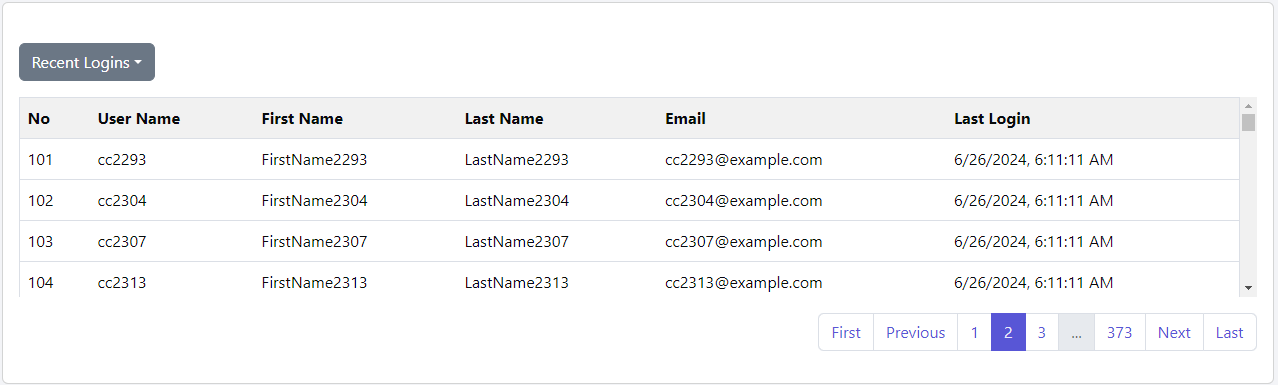
\includegraphics[width=0.8\linewidth]{list.png}
    \caption{Giao diện hiển thị danh sách thành viên trong hệ thống ASP.NET Membership}
    \label{fig:list}
\end{figure}
    